\documentclass[tikz, margin=0mm,border=0pt]{standalone}
\usepackage{tikz}
\usepackage{pgfplots}

%\pgfplotsset{compat=1.15}
\begin{document}
  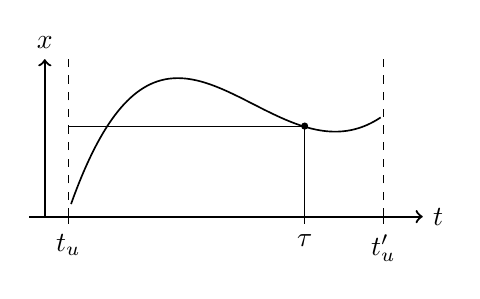
\begin{tikzpicture}[scale=1]
    \begin{axis}[hide axis,
      at = {(0.14cm,0)},
      samples     = 200,
      width=6.3cm,
      height=3.5cm,
      domain=0:pi
    ]
    \addplot[black, semithick, mark=none]{0.5-0.1*sin(x*180/pi) + 0.05*(x-1)*(x-1.5)*(x-4))};
   \end{axis}
    \draw[->, thick] (0,0) -- (5,0) node (xaxis) [right] {$t$} ;
    \draw[->, thick] (0.2,0) -- (0.2,2) node (yaxis) [above] {$x$} ;
    \draw[dashed] (0.5,0) -- (0.5,2);
    \draw[dashed] (4.5,0) -- (4.5,2);
    \draw (0.5,0)-- (0.5,-0.1) node[below]{$t_u$}  ;
    \draw (4.5,0)-- (4.5,-0.1) node[below]{$t_u'$} ;
    \draw (3.5,0) -- (3.5,-0.1) node [below] {$\tau$} ;
    \draw[thin] (3.5,0) -- (3.5,1.15);
    \draw[thin] (0.5,1.15) -- (3.5,1.15);
    \draw[fill=black] (3.5,1.15) circle (0.25ex);
  \end{tikzpicture}
\end{document}
